\documentclass[12pt]{beamer}
\usepackage{resume/dhuBeamer}

\title{东华大学 dhuBeamer 模板}
\subtitle{beamer 副标题}
\author[3000ye]{黄川桂}
\institute{管院 \& 计院}
\date{\today}


\begin{document}
\maketitle

\section{为什么使用 \LaTeX 和 Beamer}

\begin{frame}{\LaTeX 和 Beamer 简介}
    \LaTeX 是一种用于排版文档的标记语言,广泛用于学术界、出版业和技术文档中。
    它以其专业的排版质量和对数学公式的支持而闻名。
    \LaTeX 使用类似编程的语法,用户通过输入文本和特定命令来描述文档结构和格式,然后通过编译生成最终的文档。

    ~\par

    Beamer 是 \LaTeX 的一个文档类,用于制作演示文稿。它提供了许多功能和样式,使用户能够轻松创建专业和漂亮的演示文稿。
    Beamer 支持幻灯片、动画、表格、数学公式等,同时具有丰富的主题和布局选项,让用户能够自定义演示文稿的外观和感觉。
\end{frame}

\begin{frame}{\LaTeX 和 PowerPoint 对比}
    \begin{table}[h]
        \centering
        \begin{tabular}{l|l}
            Microsoft\textsuperscript{\textregistered}  PowerPoint & \LaTeX \ Beamer\\
            \midrule
            字处理工具 & 专业排版软件 \\
            容易上手,简单直观 & 容易上手 \\
            所见即所得 & 所见即所想,所想即所得 \\
            高级功能不易掌握 & 进阶难,但一般用不到 \\
            处理长文档需要丰富经验 & 和短文档处理基本无异 \\
            花费大量时间调格式 & 无需担心格式,专心作者内容 \\
            公式排版差强人意 & 尤其擅长公式排版 \\
            二进制格式,兼容性差 & 文本文件,易读、稳定 \\
            付费商业许可 & 自由免费使用 \\
        \end{tabular}
    \end{table}
\end{frame}

\section{dhuBeamer 模板介绍}
\begin{frame}{模板参考}

    \begin{itemize}
        \item 模板制作参考
        \begin{itemize}
            \item \href{https://github.com/sjtug/SJTUBeamer}{SJTUBeamer}
            \item \href{https://www.overleaf.com/latex/templates/bei-da-zhong-wen-mo-ban-pku-beamer-template/kfxpbtzrqhrn}{PKU-Beamer-Template}
        \end{itemize}
        \item 模板风格参考
        \begin{itemize}
            \item \href{https://www.dhu.edu.cn/_upload/article/files/d2/8c/2137ec0c44238fd6fbd3ee28ff07/9f9b566a-67f1-4717-991f-477ee5b43acb.zip}{东华大学标准与学术 PPT 模板(2020版)}
        \end{itemize}
        \item 模板元素来源
        \begin{itemize}
            \item \href{https://www.dhu.edu.cn/bsxt/listm.htm}{东华大学标识系统}
            \item 东华大学 LOGO,背景
            \item 东华大学颜色:锦缎红,晨曦红,风帆黄,基石灰
        \end{itemize}
    \end{itemize}

\end{frame}

\begin{frame}{模板现状}

    本模板由黄川桂于2024年2月发布 v1.0 版本,已在多个平台开源:

    ~\par

    \begin{itemize}
        \item Github: \href{https://github.com/3000ye/dhuBeamer}{dhuBeamer}
        \item Overleaf: \href{https://www.overleaf.com/latex/templates/dong-hua-da-xue-dhubeamer-mo-ban/wfqjdyjjnswr}{dhuBeamer}
        \item 3000ye Blog: \href{https://3000ye.com/p/dhubeamer/}{dhuBeamer}
        \item 公众号:3000ye Blog
    \end{itemize}

\end{frame}

\section{dhuBeamer 模板使用说明}

\begin{frame}{Beamer 中的元素概览}
    \begin{figure}[H]
        \centering
        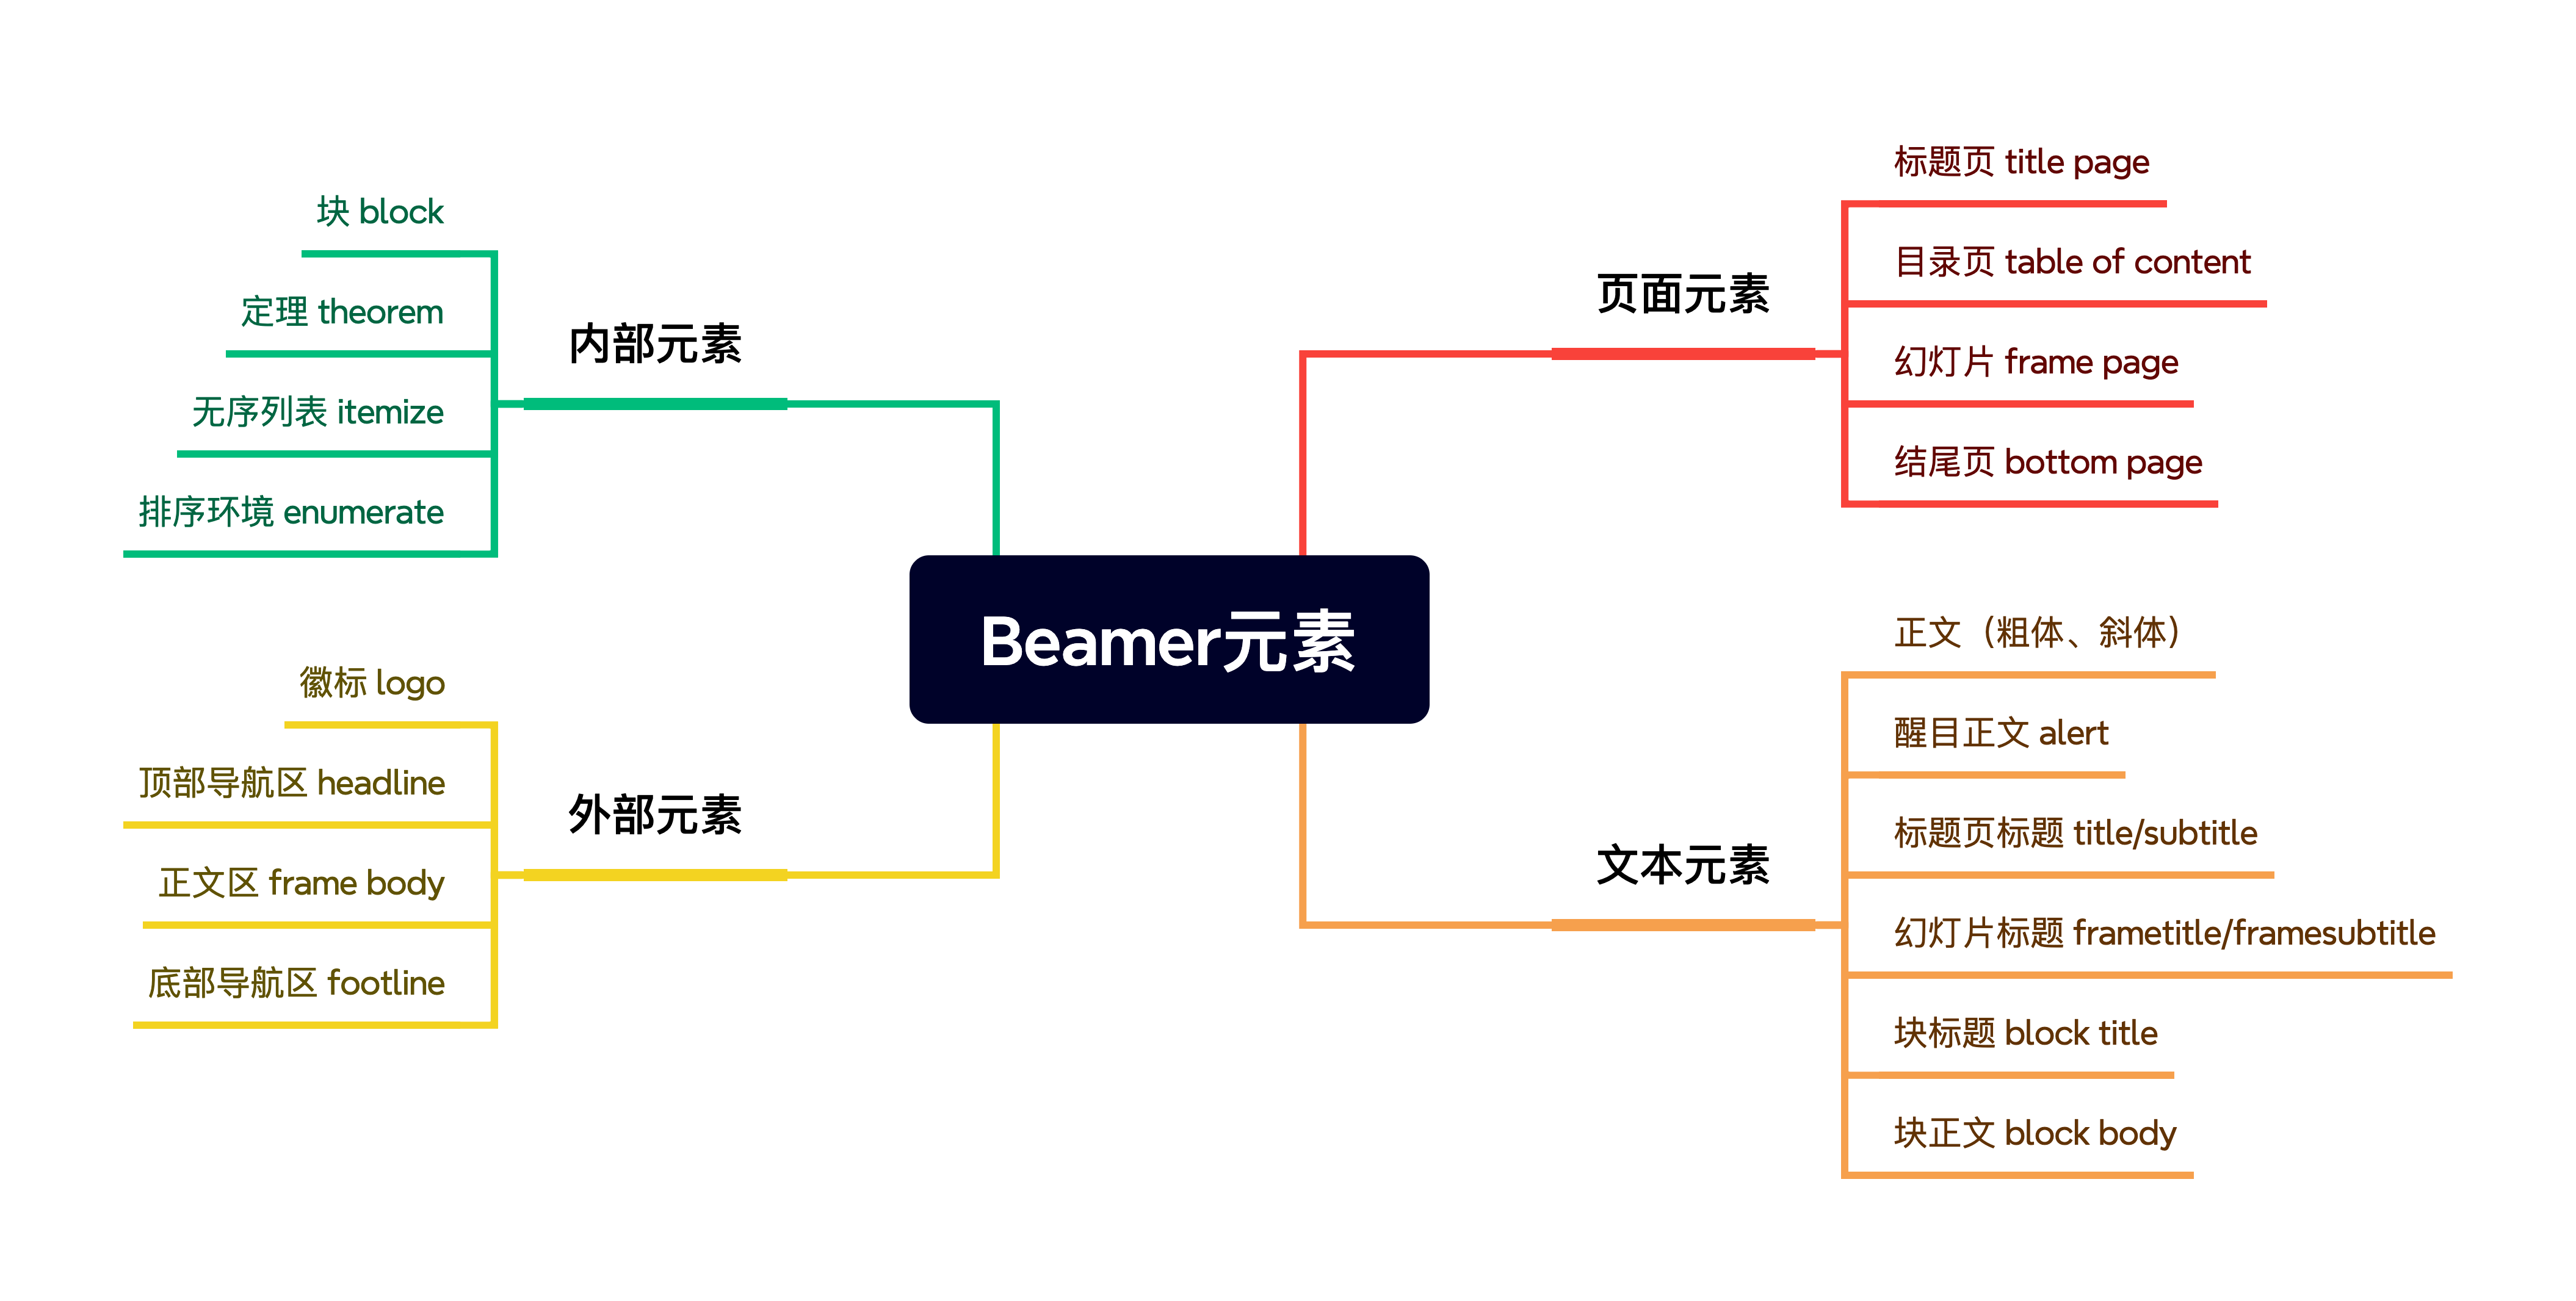
\includegraphics[width=0.85\textwidth]{assets/Beamer元素.png}
    \end{figure}
\end{frame}

\begin{frame}{\LaTeX 常用命令}
    \begin{block}{\LaTeX 常用命令}
        \centering
        \begin{tabular}{llll}
            \cmd{chapter} & \cmd{section} & \cmd{subsection} & \cmd{paragraph} \\
            章 & 节 & 小节 & 带题头段落 \\
            \hline
            \cmd{centering} & \cmd{emph} & \cmd{verb} & \cmd{url} \\
            居中对齐 & 强调 & 原样输出 & 超链接 \\
            \hline
            \cmd{footnote} & \cmd{item} & \cmd{caption} & \cmd{includegraphics} \\
            脚注 & 列表条目 & 标题 & 插入图片 \\
            \hline
            \cmd{label} & \cmd{cite} & \cmd{ref} \\
            标号 & 引用参考文献 & 引用图表公式等 \\
            \hline
        \end{tabular}
    \end{block}
\end{frame}

\begin{frame}{\LaTeX 常用环境}
    \begin{block}{\LaTeX 常用环境}
        \centering
        \begin{tabular}{lll}
            \env{table} & \env{figure} & \env{equation} \\
            表格 & 图片 & 公式 \\
            \hline
            \env{itemize} & \env{enumerate} & \env{description} \\
            无编号列表 & 编号列表 & 描述 \\
            \hline
        \end{tabular}
    \end{block}
\end{frame}

\begin{frame}{标题页与结尾页}
    \begin{columns}[T,onlytextwidth]
        \begin{column}{0.48\textwidth}
            \begin{block}{参数配置}
                \begin{itemize}
                    \item 全局标题:\env{title}
                    \item 全局副标题:\env{subtitle}
                    \item 作者:\env{author}
                    \item 学院(组织):\env{institute}
                    \item 日期:\env{date}
                \end{itemize}

                ~\par
                \alert{注意}:上述参数需放置于导言区
            \end{block}
        \end{column}
        
        \begin{column}{0.48\textwidth}
            \begin{block}{使用示例}
                \texttt{$\backslash$begin\{document\}} \par
                \hspace{2em} {\footnotesize \% 导入标题页} \par
                \hspace{2em} \texttt{$\backslash$maketitle} \par
                \hspace{4em} $\cdots \cdots$ \par
                \hspace{2em} {\footnotesize \% 导入结尾页(可自定义结尾内容)} \par
                \hspace{2em} \texttt{$\backslash$makebottom\{\}}
                \texttt{$\backslash$end\{document\}}
            \end{block}
        \end{column}
    \end{columns}
\end{frame}

\begin{frame}{列表环境}
    \begin{columns}[T,onlytextwidth]
        \begin{column}{0.48\textwidth}
            \begin{block}{无序列表}
                \begin{itemize}
                    \item 第一级
                    \begin{itemize}
                        \item 第二级
                        \item 第二级
                        \begin{itemize}
                            \item 第三级
                            \item 第三级
                        \end{itemize}
                    \end{itemize}
                    \item 第一级
                    \begin{itemize}
                        \item 第二级
                        \item 第二级
                    \end{itemize}
                    \item 第一级
                \end{itemize}
            \end{block}
        \end{column}
        
        \begin{column}{0.48\textwidth}
            \begin{block}{有序列表}
                \begin{enumerate}
                    \item 第一级
                    \begin{enumerate}
                        \item 第二级
                        \item 第二级
                        \begin{enumerate}
                            \item 第三级
                            \item 第三级
                        \end{enumerate}
                    \end{enumerate}
                    \item 第一级
                    \begin{enumerate}
                        \item 第二级
                        \item 第二级
                    \end{enumerate}
                    \item 第一级
                \end{enumerate}
            \end{block}
        \end{column}
    \end{columns}
\end{frame}

\begin{frame}{数学公式}
    \begin{columns}[T,onlytextwidth]
        \begin{column}{0.48\textwidth}
            \begin{block}{行内公式与跨行公式}
                行内公式:$\mathcal{F}(\xi)=\int_{-\infty}^{\infty} f(x)\mathrm{e}^{-\mathrm{j}2\pi
                \xi x}\,\mathrm{d}x$

                ~\par

                跨行公式:
                $$
                \mathcal{F}(\xi)=\int_{-\infty}^{\infty} f(x)\mathrm{e}^{-\mathrm{j}2\pi\xi x}\,\mathrm{d}x
                $$
            \end{block}
        \end{column}
        
        \begin{column}{0.48\textwidth}
            \begin{block}{无编号与有编号公式}
                无编号公式:
                \begin{equation*}
                    \mathcal{F}(\xi)=\int_{-\infty}^{\infty} f(x)\mathrm{e}^{-\mathrm{j}2\pi
                    \xi x}\,\mathrm{d}x
                \end{equation*}

                有编号公式:
                \begin{equation}
                    \mathcal{F}(\xi)=\int_{-\infty}^{\infty} f(x)\mathrm{e}^{-\mathrm{j}2\pi
                    \xi x}\,\mathrm{d}x
                \end{equation}
            \end{block}
        \end{column}
    \end{columns}
\end{frame}

\begin{frame}{插入单张表格}
    \begin{table}[H]
        \centering
        \caption{表格标题}
            \begin{tabular}{c||l}
            \toprule
            parameter  & Description \\
            \midrule
            $I$ & Land area collection \\
            $J$ & Flower pollination demand set \\
            $D_j$ & Number of pollinating bees required for flower pollination \\
            $T_k$ & Honeycomb size grade, $k = 1, 2, \cdots$ \\
            $B$ & Maximum number of hive \\
            $R_{ik}$ & Maximum influence radius of a single honeycomb \\
            \bottomrule
            \end{tabular}%
        \label{tab: 一个表}%
    \end{table}%
\end{frame}

\begin{frame}{插入多张表格}
    \begin{minipage}[c]{0.45\textwidth}
        \centering
        \begin{table}[H]
            \centering
            \caption{表格1标题}
                \begin{tabular}{c||lc}
                \toprule
                Symbol  & Description & Unit \\
                \midrule
                $t$ & $t_{th}$ year & $\sim$ \\
                $e_k$ & the error term & $\sim$ \\
                $X_{ij}$ & Raw data matrix & $\sim$ \\
                $Y_{ij}$ & Positive matrix & $\sim$ \\
                \bottomrule
                \end{tabular}%
            \label{tab: 表格1标题}%
        \end{table}%
    \end{minipage}
    \begin{minipage}[c]{0.45\textwidth}
        \centering
        \begin{table}[H]
            \centering
            \caption{表格2标题}
                \begin{tabular}{c||lc}
                \toprule
                Symbol  & Description & Unit \\
                \midrule
                $t$ & $t_{th}$ year & $\sim$ \\
                $e_k$ & the error term & $\sim$ \\
                $X_{ij}$ & Raw data matrix & $\sim$ \\
                $Y_{ij}$ & Positive matrix & $\sim$ \\
                \bottomrule
                \end{tabular}%
            \label{tab: 表格2标题}%
        \end{table}%
    \end{minipage}
\end{frame}

\begin{frame}{插入单张图片}
    \begin{figure}[H] % 图片位于文字下方
        \centering % 居中
        % 设置图片占页面宽度的比例(默认0.8)
        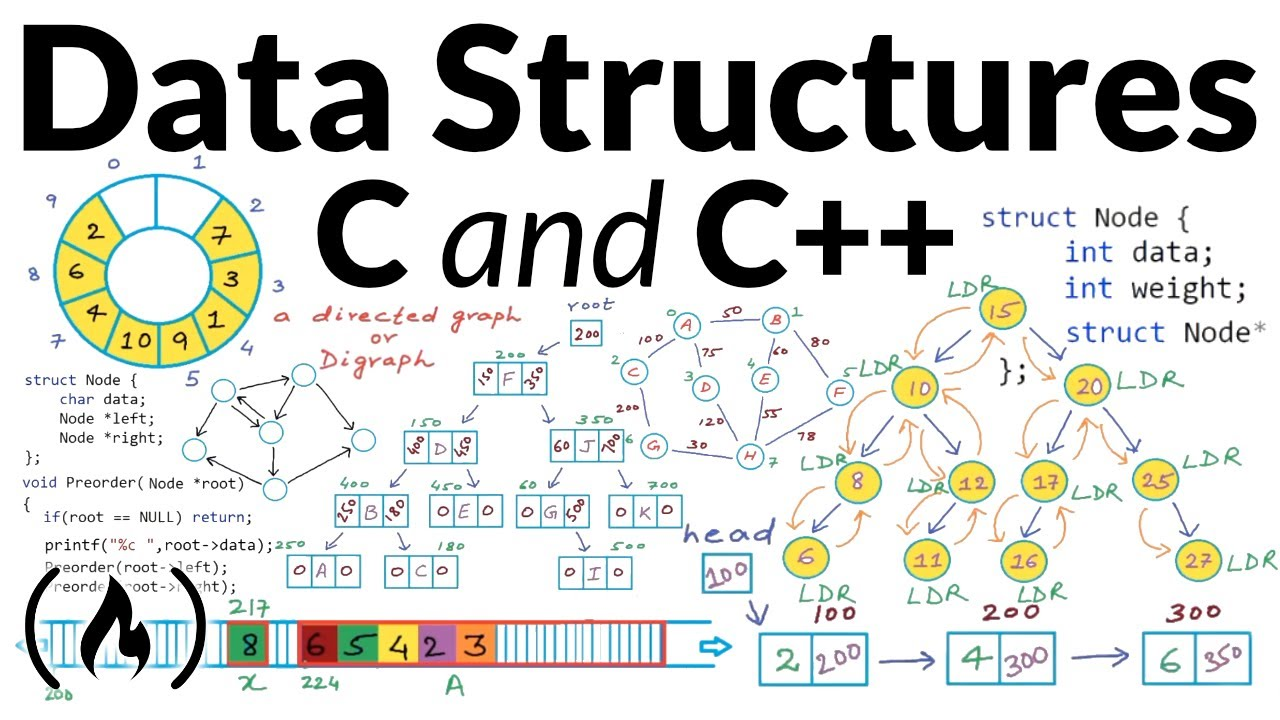
\includegraphics[width=0.6\textwidth]{assets/dataStructures.jpg}
        \caption{图片标题} % 图例,按章节编号
        \label{fig: 数据结构2} % 图片索引
    \end{figure}
\end{frame}

\begin{frame}{插入多张图片}
    \begin{figure}[H]
        \centering
        \begin{minipage}[c]{0.40\textwidth} %minipage使之保持同一行
        \centering
        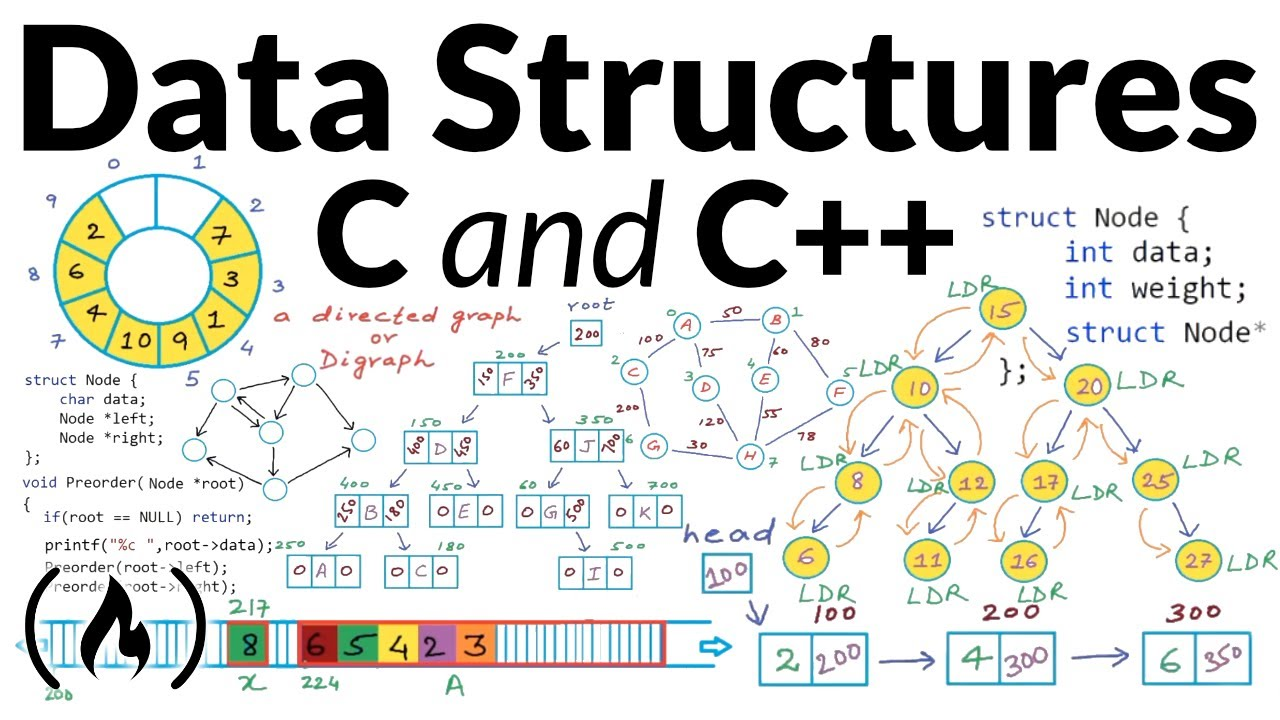
\includegraphics[width=0.8\textwidth]{assets/dataStructures.jpg}\\
        \caption{图片1标题}
        \end{minipage}
        \hspace{1em}
        \begin{minipage}[c]{0.40\textwidth} %minipage使之保持同一行
        \centering
        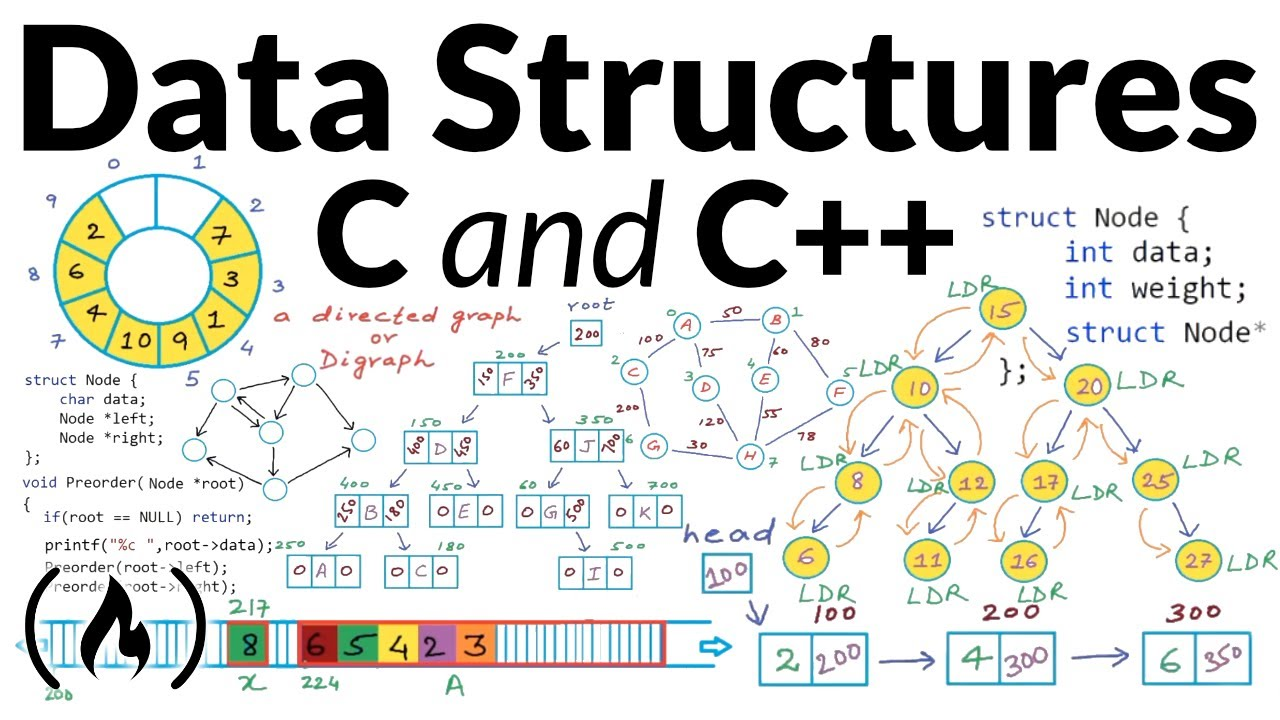
\includegraphics[width=0.8\textwidth]{assets/dataStructures.jpg}\\
        \caption{图片2标题}
        \end{minipage}
    \end{figure}
\end{frame}

\begin{frame}{插入参考文献}
    考虑到在 Slides 中插入文献的需求并不高,
    因此这里只提供手动管理文献的方案,如需使用 bibTex 请自行查阅资料。

    ~\par

    \begin{thebibliography}{99}
        \bibitem{RN1} 参考文献
        \bibitem{RN2} 参考文献
    \end{thebibliography}
\end{frame}

\makebottom{感谢使用 dhuBeamer 模板}
\end{document}
